\subsection{Структурный фактор рассеяния}
\label{sec:structure_factor}
Атомы решетки излучают рассеянное электромагнитное излучение.
Если в элементарной ячейке более одного атома, волны от разных атомов,
 интерферируя между собой, вносят вклад в общую картину рассеяния,
 ослабляя или усиливая ее.

 \begin{figure}[H]
   \centering
   \subfloat[Коструктивная интерференция]{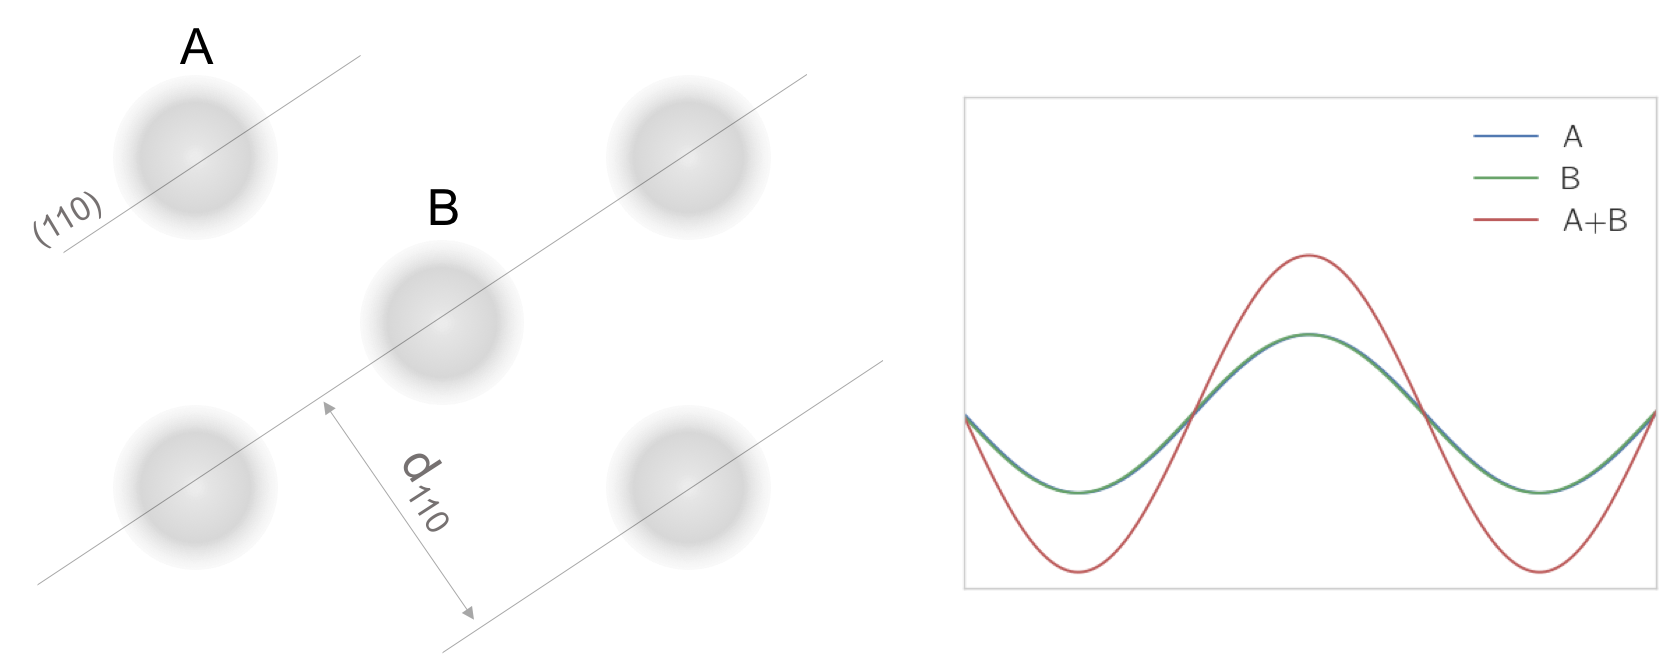
\includegraphics[width=0.45\textwidth]{images/interference_construct.png}\label{fig:f1}}
   \hfill
   \subfloat[Деструктивная интерференция]{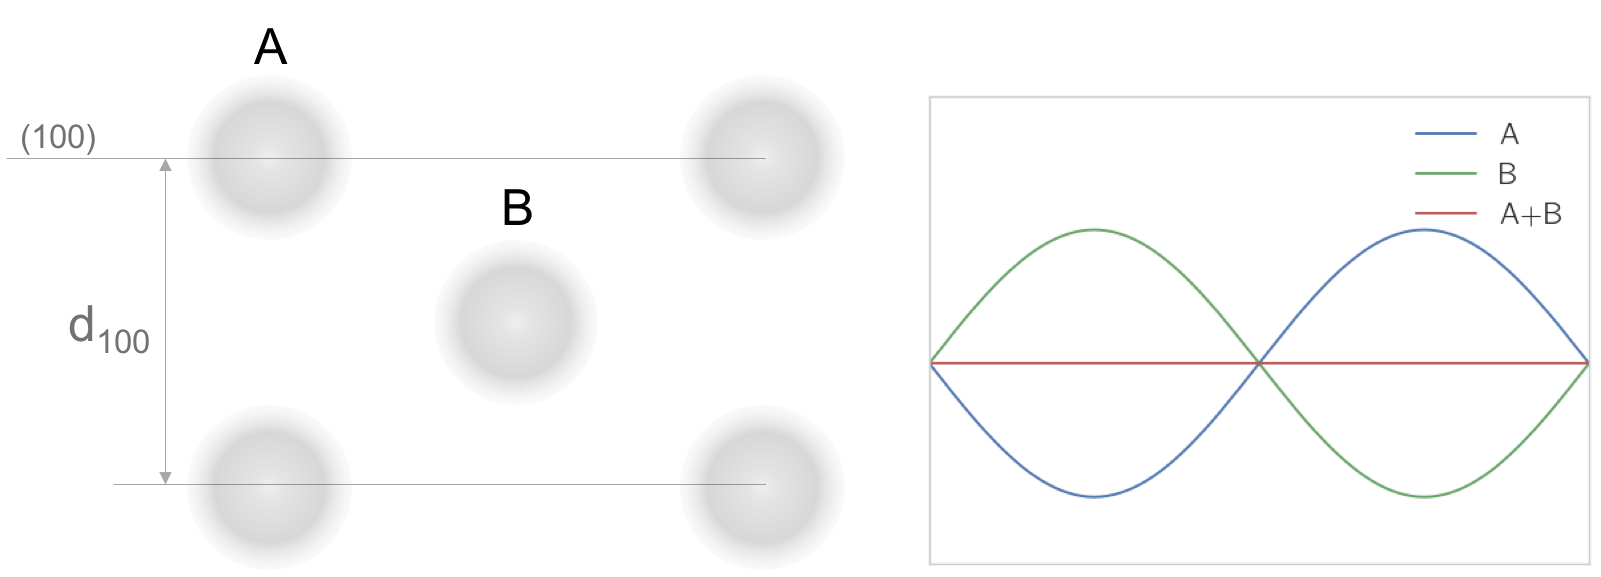
\includegraphics[width=0.45\textwidth]{images/interference_destruct.png}\label{fig:f2}}
   \caption{Примеры интерференции двух волн, отраженных соседними атомными плоскостями}
   \label{ris:interference_by_plate}
 \end{figure}

Рассеяние от набора атомов характеризуется структурным фактором рассеяния,
 с учетом векторного сложения всех фаз по всем атомам N элементарной ячейки:

 \begin{equation}
   F = \sum_{n} f_n e^{ i\vec{h}\vec{r}_n} =   \sum_{n} f_n \cdot e^{-i\phi_n}
  \end{equation}

  где $\phi_n = 2 \pi (hx_n+ky_n+lz_n)$.


На рисунке ~\ref{ris:hkl_LGT_SI} цветом изображена величина структурного фактора для разных
 индексов плоскостей отражения в сравнении между кристаллом LGT и Si.
 В таком представлении просматривается периодичность образования запрещенных
 рефлексов в кубическом кремнии. В кристалле LGT запрещенных (синий цвет)
  индексов для отражения на порядок меньше, связанно это с более низкими
  симметричными свойствами.

  \begin{figure}[h]
    \centering
    \subfloat[кристалл Si]{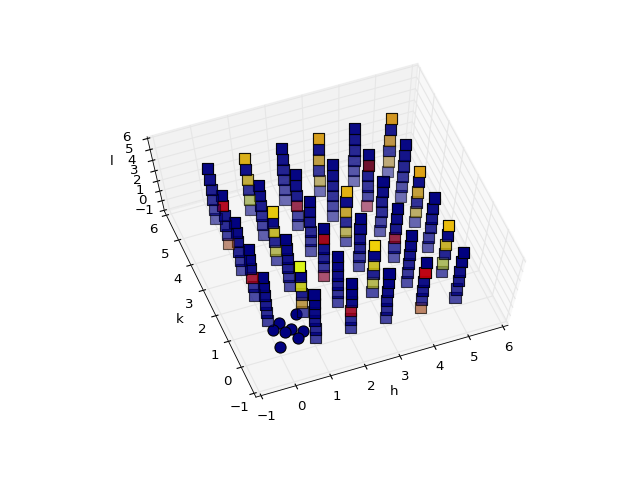
\includegraphics[width=0.5\textwidth]{images/hkl_Si.png}}
    \hfill
    \subfloat[кристалл LGT]{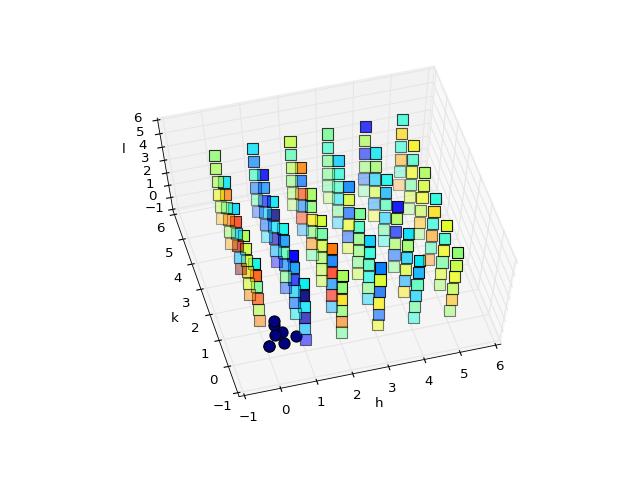
\includegraphics[width=0.5\textwidth]{images/hkl_LGT.png}}
    \caption{Карта распределения величины структурного фактора
    (цвет соответствует его величине) в координатах индексов Миллера}
    \label{ris:hkl_LGT_SI}
  \end{figure}
